\documentclass[11pt]{article}

\usepackage{float}
\usepackage{hyperref}
\usepackage{fullpage}
\usepackage{verbatim}
\usepackage{moreverb}
\usepackage{graphicx}
\usepackage{parskip}
\usepackage{tikz}
\usetikzlibrary{arrows,automata, positioning}
\usepackage{minted}
\let\verbatiminput=\verbatimtabinput
\def\verbatimtabsize{4\relax}

\begin{document}
\title{EECS 151/251A FPGA Lab\\
Lab 3: Rotary Encoder and Debouncer, Finite State Machines, Synchronous Resets, Synchronous RAM, Testbench Techniques}

\author{Prof. Elad Alon \\
TAs: Vighnesh Iyer, Bob Zhou \\Department of Electrical Engineering and Computer Sciences\\
College of Engineering, University of California, Berkeley}
\date{}
\maketitle

\tableofcontents

\section{Before You Start This Lab}

Before you proceed with the contents of this lab, we suggest that you review these documents that will help you better understand some concepts we will be covering.

\begin{enumerate}
	\item \textbf{labs\_fa16/docs/Verilog/verilog\_fsm.pdf}
	
	Goes over concepts of FSM in Verilog. Provides an example of implementing FSM's in Verilog and pitfalls to watch out for.
	
	%\item \url{http://www.labbookpages.co.uk/electronics/debounce.html}
	%Read the "What is Switch Bounce" section to get idea of why we need a debouncer circuit. Read the "Digital Switch Debouncing" section to get a general overview of the circuit, its parts, and their purposes. You may want to pay attention to the purpose of the synchronizer as meta-stability is something you will go over in class.
	
	%\item \url{http://www.xilinx.com/products/boards/s3estarter/files/s3esk_rotary_encoder_interface.pdf}
	
	%Read slide 5 (Rotary Encoder and Signals) to get an idea of how the encoder works and the signal it generates. You can read the next few pages to get a better idea of how to use the signals. You will be implementing the circuit described in these slides in this lab.

\end{enumerate}

\section{Lab Overview}

In this lab, we will learn about circuits to take the signals generated by the buttons and rotary encoder on the ML505 board and convert them into a digital signal we can use in our FPGA design. You will be using the LED's to confirm that your input conditioning circuits are working correctly. We will discuss how to use synchronous resets to reset our circuits to a known initial state. We will be creating a basic FSM in the \verb|music_streamer| that uses the buttons and rotary encoder to change states and alter the music playback.

Run \verb|git pull| in your \textbf{git cloned} \verb|labs_sp17| directory to fetch the latest skeleton files for this lab.

\section{Synchronizer, Debouncer, and Rotary Encoder}

%\begin{center}
%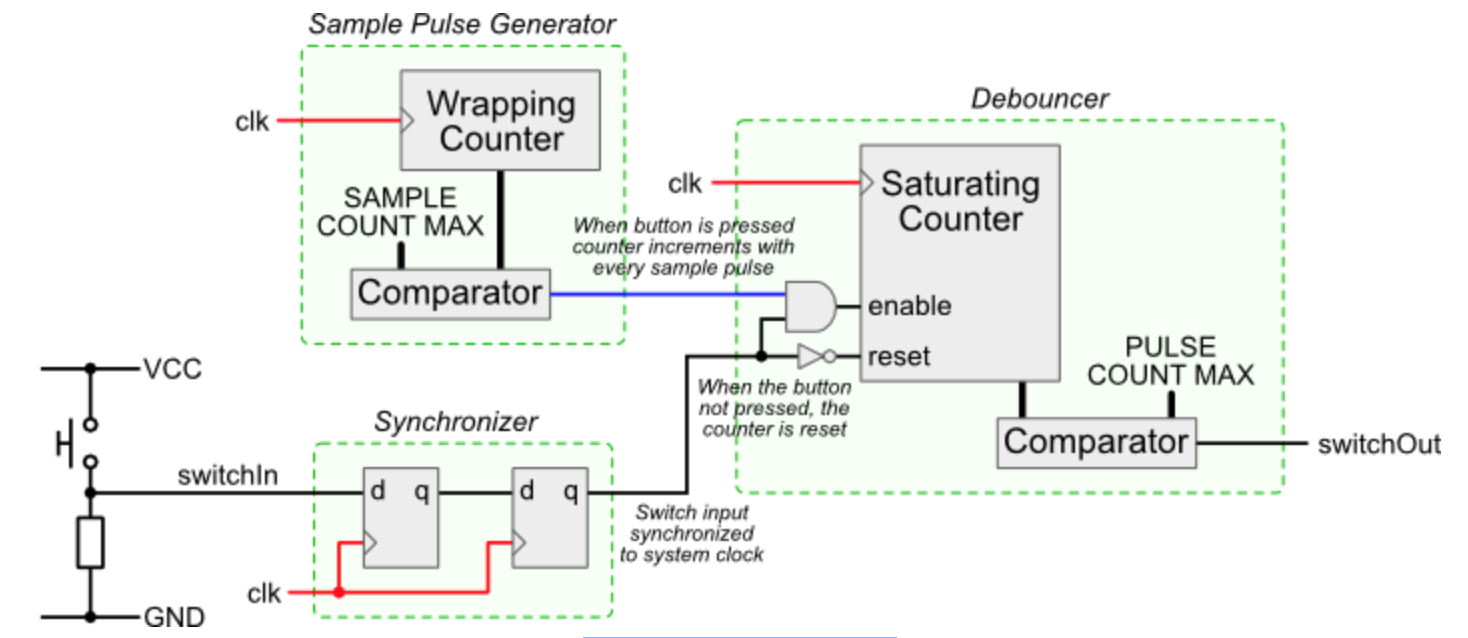
\includegraphics[height=5cm]{images/lab2_fig2.png}
%\end{center}

%Recall this graphic from the prelab debouncer reading. It is an overview of the debouncer circuit which includes the synchronizer circuit.

\subsection{Synchronizer}
In Verilog (RTL), digital signals are either 0's or 1's. In a digital circuit, a 0 or 1 corresponds to a low or high voltage. If the circuit is well designed and timed (fully synchronous), we only have to worry about the low and high voltage states, but in this lab we will be dealing with asynchronous signals.

The signals coming from the push buttons and rotary encoder on the ML505 board don't have an associated clock signal. Thus, when those signals are put through a register, the hold or setup time constraints of that register may be violated. This may put that register into a \textbf{metastable} state.

\begin{figure}[H]
	\centerline{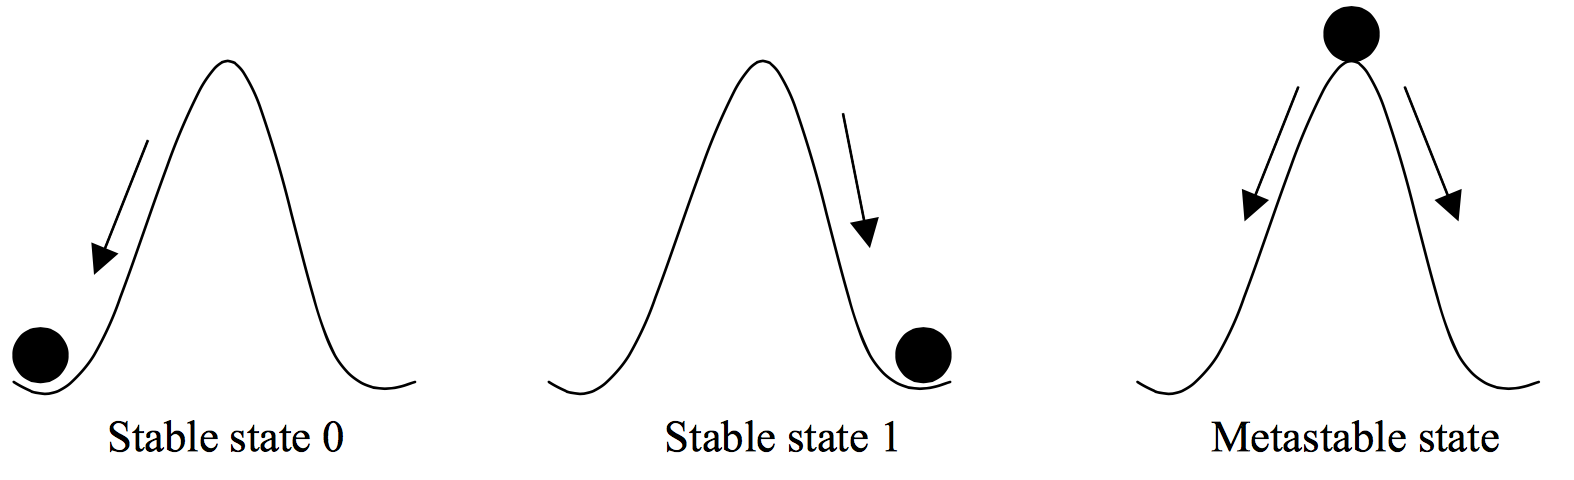
\includegraphics[height=3cm]{images/lab2_fig3.png}}
	\caption{The 'ball on a hill' metaphor for metastability. If a register's timing constraints are violated, its output voltage oscillates and after some time unpredictably settles to a stable state.}
\end{figure}

In a fully synchronous circuit, the timing tools will determine the fastest clock frequency under which the setup time constraints are all respected and the routing tools will ensure that any hold time constraints are handled. Introducing an asynchronous signal that isn't changing with respect to a clock signal can cause a register to go into a metastable state. This is undesirable since this will cause a 'mid-rail' voltage to propagate to other logic elements and can cause catastrophic timing violations that the tools never saw coming.

We will implement a synchronizer circuit that will safely bring an asynchronous signal into a synchronous circuit. The synchronizer needs to have a very small probability of allowing metastability to propagate into our synchronous circuit.

This synchronizer circuit we want you to implement for this lab is relatively simple. For synchronizing one bit, it is a pair a flip-flops connected serially. This circuit synchronizes an asynchronous signal (not related to any clock) coming into the FPGA. We will be using our synchronizer circuit to bring any asynchronous off-FPGA signals into the clock domain of our FPGA design.

\begin{figure}[H]
	\vspace{0.5cm}
	\centerline{\includegraphics[height=2.5cm]{images/Synchronizer.png}}
	\caption{1-bit 2 Flip-Flop Synchronizer}
\end{figure}

Edit the \verb|lab3/src/synchronizer.v| file to implement the two flip-flop synchronizer. This module is parameterized by a \verb|width| parameter which indicates the number of one-bit signals to synchronize.

\subsubsection{Testing in Simulation}
The testbenches to be run are stored in \verb|lab4/sim/tests|. Each \verb|.do| file in this directory is run when you run \verb|make| in the \verb|lab4/sim| directory. If you only want to run one testbench, you can rename all the other \verb|.do| files in this directory to have a different file extension.

Run \verb|make| in the \verb|lab4/sim| directory to run the testbenches. We have provided a testbench for your synchronizer called \verb|sync_testbench| in \verb|lab4/src/sync_testbench.v|. Take a look at the code for this testbench and run it; \textbf{the testbench should pass and you should inspect the waveform before you move on.} For details on the techniques/syntax used in this testbench, refer to Section 7 of this lab.

%\subsubsection{Testing on the FPGA}
%As a rudimentary test of your synchronizer, we have provided a file called \verb|lab4/src/synchronizer_fpga_test.v| which will synchronize various button press signals and send them to the GPIO LEDs. Execute the following commands:

%\begin{minted}[frame=single]{bash}
%make TOP=synchronizer_fpga_test
%make TOP=synchronizer_fpga_test report
%make TOP=synchronizer_fpga_test impact
%\end{minted} 

%We are changing the default value of \verb|TOP| that the \verb|Makefile| uses, to point to \verb|synchronizer_fpga_test| as the top level module rather than \verb|ml505top|. This allows us to build and impact different top level modules in the same folder. Keep in mind that each top level module needs a UCF file with the same name defining its I/O.

%Take a look at this test module and try it out on the board. Pressing various buttons should light up their respective LEDs. \\

%You will notice that when pressing certain buttons, the LED flickers on and off before setting at on. This can create issues in our digital logic if we just assume that a low to high logic level transition constitutes a button press, since we will get erroneous presses. We use a debouncer to fix this issue.

\subsection{Debouncer and Edge Detector}

For this lab, the debouncer circuit will take a button's digital input and output a single pulse indicating a single button press. The reason we need a somewhat involved circuit for this is shown in the figure below.

\begin{center}
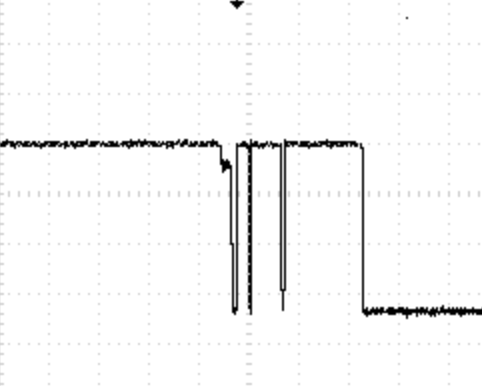
\includegraphics[height=5cm]{images/lab2_fig4.png}
\end{center}

When we press the button, we don't get a perfect stable signal. Instead the button signal has a mechanical 'bounce'. A debouncer turns this waveform, which shows a single button press, into a single pulse that our circuit can use.

Take a look at \verb|lab4/src/debouncer.v|. This is a parameterized debouncer which can debounce \verb|width| signals at a time. Your debouncer receives a vector of synchronized 1-bit signals and it outputs a debounced version of those signals. The other parameters reference the constants used in the circuit from the prelab reading.

The debouncer consists of:

\begin{enumerate}
	\item \textbf{Sample Pulse Generator} - Tells our main debouncer counter when to sample the input signal. It should output a 1, every \verb|sampling_pulse_period| clock cycles. By default \verb|sampling_pulse_period| is set to 25000.
	
	\item \textbf{Saturating Counter} - This is a counter that counts up to \verb|saturating_counter_max|. The saturating counter should increment by one every time the input signal is 1 and the sample pulse generator tells us to sample the input signal. At any clock edge, if the input signal is 0, the saturating counter should be reset to 0. Once the saturating counter reaches \verb|saturating_counter_max|, it should hold that value indefinitely until the input signal falls to 0, upon which the saturating counter should be reset to 0. The output of your debouncer should be an equality check between the saturating counter and \verb|saturating_counter_max|.
\end{enumerate}

You will likely need to use 2D regs in Verilog to implement a saturating counter for each input signal to debounce. You will also likely need to use generate-for. You can use the same sample pulse generator for all input signals.

Here is an example of creating a 2D array and using a generate-for loop:

\begin{minted}{verilog}
reg [7:0] arr [0:3]; // 4 x 8 bit array
arr[0]; // First byte from arr (8 bits)
arr[1][2]; // Third bit of 2nd byte from arr (1 bit)

genvar i;
generate
	for (i = 0; i < width; i = i + 1) begin:LOOP_NAME
		always @ (posedge clk) begin
			// Insert synchronous Verilog here
		end
	end
endgenerate
\end{minted}

\subsubsection{Debouncer Clarifications For Lab 4}
To clarify, you should use the same sample pulse generator for all input signals into your debouncer, but you should have a separate saturating counter per input signal. \\

%Last lab, there were some questions about using an array for the debouncer. We will elaborate more and review the debouncer circuit so there is less confusion this time. 

%The debouncer for one button uses two counters. Let us start with the saturating counter. The saturating counter receives two essential signals: the synchronized input and an enable signal. Every time the enable signal goes high, one of the two things can happen:
%\begin{itemize}
%\item if the synchronized input signal was high, we increment the counter. Once this counter equals \verb|PULSE_COUNT_MAX|, we indicate the button has been pressed long enough. The larger \verb|PULSE_COUNT_MAX| is, the longer we have to hold the button for the circuit to realized we actually pushed the button.
%\item if the input synchronized signal was low, we reset the counter. This essentially means we stopped pressing the button before the circuit realized we pushed the button.
%\end{itemize}

%The wrapping counter essentially tells the saturating counter when to count. Everything we reach \verb|SAMPLE_COUNT_MAX|, we tell the saturating counter to count by one For example, if we made \verb|SAMPLE_COUNT_MAX| equal to 1, we'd be telling the saturating counter to count or reset every cycle. 

%The reason we had an array was because we have multiple buttons. Each button will at the very least need its own saturating counter. We don't want the counter of one button affecting the others. The sampling counter doesn't necessarily need multiple counters because it can tell all saturating counters to sample at the same time and this won't cause them to interfere with one another. We could have had a separate wire for each counter but we wanted you to make the module parameterizable. Thus we use an array whose size can be adjusted with a parameter and one row of the array represents one of the saturating counters for one of your buttons. 

%The issue in this lab is that the debouncer of your button outputs a one clock period wide pulse at an edge while your rotary encoder circuit expects the signal to be high much longer. Part of the rotary encoder circuit expects both the incoming signal from the wheel to be high at some point so we cannot just have a one clock period wide pulse when we detect that one of the signals from the wheel have gone high.

*Note: Some of you have been asking about the widths of the counters used in the debouncer circuit. We provided a log base 2 macro that will calculate the number of binary bits needed to represent a decimal number. 

\subsubsection{Edge Detector}

The debouncer we created in the last lab (Lab 3) had an implicit edge detector: we gave you the specifications of the module and you implemented it as one block. In this lab, we will intentionally decouple the edge detector from the debouncer. An edge detector will take an input signal and will output a one clock period wide pulse on a rising edge of the input signal.

You will feed the output of your button debouncer through an edge detector before passing the signal to the \verb|music_streamer| or reset net.

Create a variable-width edge detector in \verb|lab4/src/edge_detector.v|. 

\subsubsection{Testing in Simulation}

We've provided a testbench to test your debouncer and edge detector circuits in \verb|lab4/src/debouncer_testbench.v| and \verb|lab4/src/edge_detector_testbench.v|. Run the testbench, make sure it passes, and inspect the waveforms before FPGA testing.

\subsubsection{Testing on the FPGA}
We have created a top level module called \verb|debouncer_fpga_test| that will create a 8-bit register and will use button presses to add and subtract from it. This module will use both your \verb|debouncer.v| and \verb|edge_detector.v|.

Pressing any button will cause the register to increment and the LEDs will show the current value of the register. Pressing the South compass button however, will cause the register to decrement.

\begin{minted}[frame=single]{bash}
make TOP=debouncer_fpga_test
make TOP=debouncer_fpga_test report
make TOP=debouncer_fpga_test impact
\end{minted} 

Make sure that your report gives you \textbf{zero warnings for synthesis.} You must fix any and all warnings before your debouncer will work well on the FPGA.\\

\textbf{Show the TA the debouncer working before moving on. It is critical that your debouncer works properly.}

You will discover when playing with your debouncer that the buttons have a way that they like being pressed to minimize bounce; get a good feel for them.

\subsection{Rotary Encoder}

The rotary encoder consists of a circuit that has two switches that go high as you rotate the wheel. Recall this waveform from the prelab reading.

\begin{center}
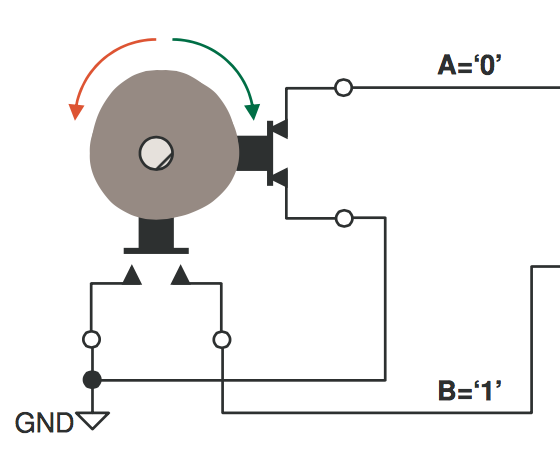
\includegraphics[height=5cm]{images/lab2_fig5.png}
\end{center}

Our main concern is finding out which direction the wheel turned. The following oscilloscope waveform from the prelab reading illustrates how we will do so. 

\begin{center}
	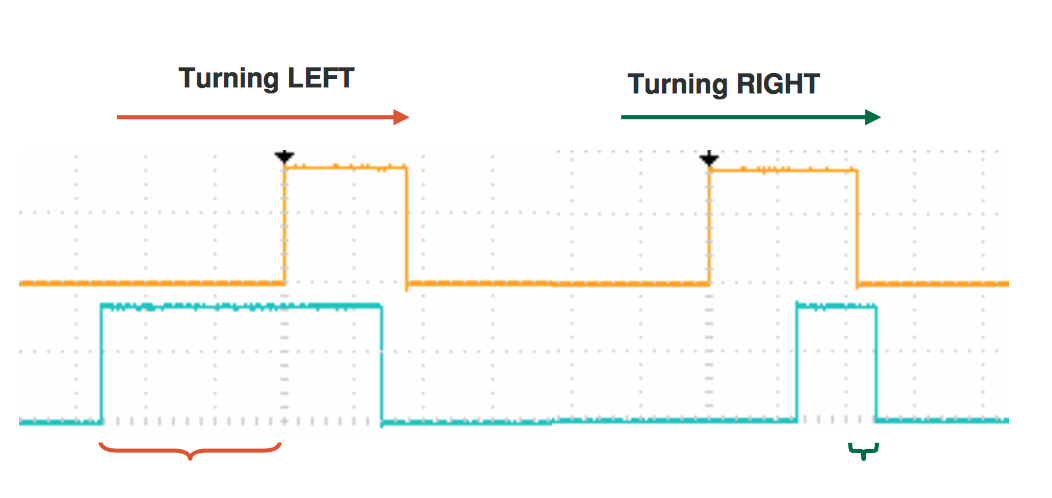
\includegraphics[height=5cm]{images/lab2_fig6.png}
\end{center}

If the pulse from A (top wave - orange) happens before the pulse from B (bottom wave - blue), it indicates that a the wheel has been turned a certain way. If the wheel is spun in the opposite direction then B's pulse will occur before A. We will take advantage of the fact that we can examine the logic level of wave B at the rising edge of wave A to determine direction of wheel movement.\\

Open up \verb|lab3/src/rotary_decoder.v|. This module takes the synchronized A and B signals, and a clock input. It outputs \verb|rotary_event| when a wheel click has been detected and \verb|rotary_left| indicates whether that spin was to the right or the left.\\

Begin by implementing the Rotary Contact Filter as described in slide 7 of the prelab reading. This is a simple filter to remove glitching from the A and B signals. After implementing the filter, refer to slide 8 of the prelab reading for the circuit that will produce the \verb|rotary_event| and \verb|rotary_left| outputs.

\subsubsection{Testing in Simulation}
We have provided a rotary decoder testbench for you in \verb|lab4/src/rotary_decoder_testbench.v|. Run this testbench and make sure it passes; inspect the waveforms. Proceed to the FPGA test once you have confirmed expected behavior in simulation.

\subsubsection{Testing on the FPGA}
There is a test top level module called \verb|rotary_decoder_fpga_test|. It allows you to spin the rotary encoder to increment and decrement a 8-bit counter whole value is shown on the GPIO LEDs. Pushing the rotary encoder button will cause the counter to reset it to 0. Run it as such.

\begin{minted}[frame=single]{bash}
make TOP=rotary_decoder_fpga_test
make TOP=rotary_decoder_fpga_test report
make TOP=rotary_decoder_fpga_test impact
\end{minted} 

Make sure that your report gives you \textbf{zero warnings for synthesis.} You must fix any and all warnings before your rotary encoder will work well on the FPGA.\\

\textbf{Show the TA the rotary encoder working before moving on. It is critical that your rotary encoder works properly.}

Congratulations! You just built four highly useful and practical digital circuits. Now let's integrate them into our larger music streamer design.

\section{Testbench Techniques}
There are several testbenches included in this lab for your synchronizer, edge detector, rotary encoder, debouncer, and music streamer that introduce you to some useful Verilog testbench constructs.

\begin{itemize}
\item \verb|@(posedge <signal>)| and \verb|@(negedge <signal>)| - These are a different type of delay statement from what you have seen before. \verb|#10| would advance the simulation by 10 timesteps. These commands will advance the simulation until the \verb|<signal>| rises or falls.

For example:
\begin{minted}[frame=single]{verilog}
@(posedge signal);
@(posedge signal);
\end{minted}

Simulation time will advance until we have seen two rising edges of \verb|signal|.

\item \verb|repeat| - it acts like a \verb|for| loop but without an increment variable

For example:
\begin{minted}[frame=single]{verilog}
repeat (2) @(negedge clk);
repeat (10) begin 
	@(posedge clk);
end
\end{minted} 

The simulation will advance until we have seen 2 falling clock edges and will then advance further until we have seen 10 rising clock edges.

\item \verb|$display| - acts as a print statement. Similar to languages like C, if you want to print out a wire, reg, integer, etc... value in your testbench, you will need to format the string.

For example:
\begin{minted}[frame=single]{verilog}
$display("Wire x in decimal is %d", x);
$display("Wire x in binary is %b", x);
\end{minted} 

\item \verb|tasks| - tasks are subroutines where you can essentially group and organize some commands rather than haphazardly putting them everywhere. They can take inputs and outputs. An few examples are shown in the provided testbenches.

\item \verb|fork/join| - Allows you to execute testbench code in parallel. You create a fork block with the keyword \verb|fork| and end the block with the keyword \verb|join|.

For example:
\begin{minted}[frame=single, tabsize=4]{verilog}
fork
	begin
		task1();
	end
	begin
		$display("Another thread");
		task2();
	end
join
\end{minted}

Multiple threads of execution are created by putting multiple begin/end blocks in the fork block. In this example, thread 1 runs \verb|task1()|, while thread 2 first \verb|$display|s some text then runs \verb|task2()|. The threads operate in parallel.

\item Hierarchical Paths - you can access signals inside an instantiated module for debugging purposes. This can be helpful in some cases where you want to look at an internal signal but don't want to create another output port just to look at it.

For example:
\begin{minted}[frame=single, breaklines]{verilog}
tone_generator tone_gen ();
$display("Signal inside my tone_generator instance, clock_counter: %b", tone_gen.clock_counter);
\end{minted} 
\end{itemize}

\section{Synchronous Resets In Design and Simulation}
Now that we have a debouncer that can give us a pulse for a press of a button, we have a way of explicitly resetting our circuits! You will recall that in the previous lab, we set the initial value of registers as below so that our simulation would have defined signals.

\begin{minted}{verilog}
reg [23:0] clock_counter = 0;
\end{minted}

Now that we have a reset signal tied to the CPU\_RESET push button, we can do this instead.

\begin{minted}{verilog}
always @ (posedge clk) begin
	if (rst) begin
		clock_counter <= 24'd0;
	end
end
\end{minted}

Unlike what we did before, this RTL is synthesizable for all deployment targets, FPGAs, ASICs, and CPLDs alike. Go ahead and modify your \verb|tone_generator| and \verb|music_streamer| to use the provided reset signal to get your registers to a default state. You might also want to modify your debouncer, synchronizer, edge detector, and rotary decoder to use the provided reset signal.

After doing this, run the \verb|tone_generator_testbench| again using \verb|make| in the \verb|lab4/sim/| directory. View the waveform using ModelSim and see how we used a reset in the testbench to bring all the registers to a defined state without specifying a default value.

\section{Music Streamer Tempo Control}
Let's use the new user inputs we now have access to. You will recall that your \verb|music_streamer| by default chooses to play each tone in the ROM for 1/25th of a second. Extend the functionality of the \verb|music_streamer| so that spinning the rotary encoder changes the tempo of the notes. Pushing in the rotary encoder should reset the tempo back to the default value.\\

You should implement this by using a register to hold the number of clock cycles per note. Instead of this number being hardcoded in Verilog to represent $\frac{1}{25}$th of a second, you can change it at runtime. Spinning the rotary encoder once should add or subtract a fixed number from this register which should alter the time each tone is played (i.e. tempo).\\

Try this out on the FPGA and verify that you have control of your \verb|music_streamer|'s tempo using the rotary encoder. You should be able to speed up and slow down the music you are playing.

\section{Music Streamer FSM}
Now, you will implement a simple FSM in the \verb|music_streamer|. \textbf{If you've done this part in Lab 3, make sure your FSM matches this slightly modified spec}.

The FSM will have 3 states: \verb|PAUSED|, \verb|REGULAR_PLAY|, \verb|REVERSE_PLAY|. Here is the state transition diagram:

\begin{center}
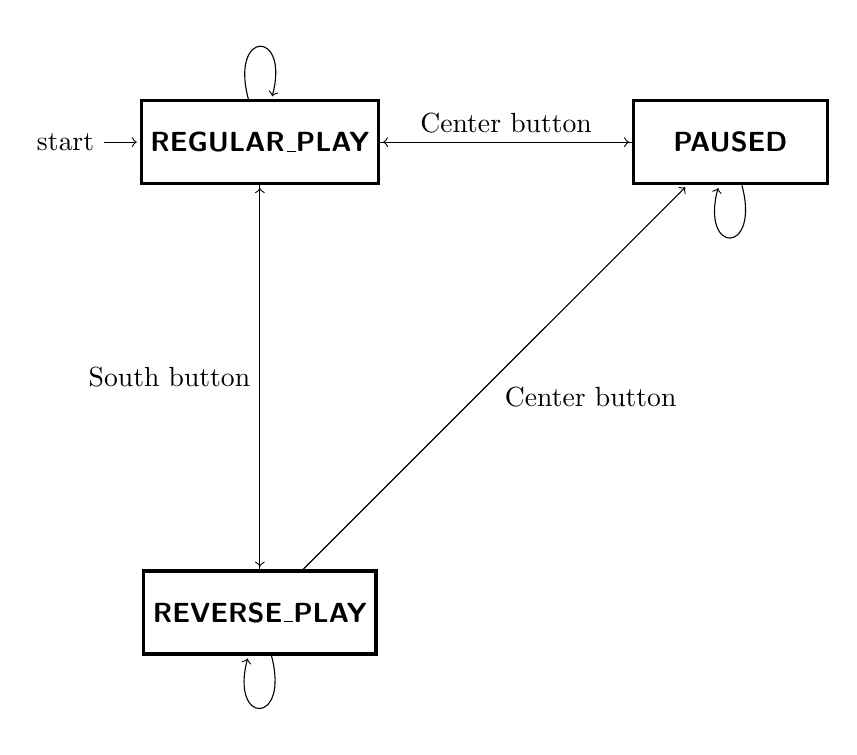
\begin{tikzpicture}[shorten >=1pt, node distance=10cm,on grid, auto]
  \tikzstyle{state} = [draw, very thick, fill=white, rectangle, minimum height=3em, minimum width=7em, node distance=17em, font={\sffamily\bfseries}]
  \tikzstyle{stateEdgePortion} = [black,thick];
  \tikzstyle{stateEdge} = [stateEdgePortion,->];
  \tikzstyle{edgeLabel} = [pos=0.5, text centered, font={\sffamily\small}];
  
	\node[state,initial](rp) {REGULAR\_PLAY};
	\node[state](revp) [below =of rp]{REVERSE\_PLAY};
	\node[state](p) [right=of rp]{PAUSED};

	\path[->]
	(rp) edge node {Center button} (p)
		edge [swap] node {South button} (revp)
		edge [loop above] node {} (rp)
	(p) edge node {} (rp)
		edge [loop below] node {} (p)
	(revp) edge [swap] node {Center button} (p)
		edge [swap] node {} (rp)
		edge [loop below] node {} (revp);
\end{tikzpicture}
\end{center}

\begin{enumerate}
	\item Your initial state should be \verb|REGULAR_PLAY|. 
	
	\item Pressing the center compass push button should transition you into the \verb|PAUSED| state from either the \verb|REGULAR_PLAY| or \verb|REVERSE_PLAY| states. Pressing the center compass push button while in the \verb|PAUSED| state should transition the FSM to the \verb|REGULAR_PLAY| state.
	
	\item In the \verb|PAUSED| state, your ROM address should be held steady at its value before the transition into \verb|PAUSED| and no sound should come out of the piezo speaker. After leaving the \verb|PAUSED| state your ROM address should begin incrementing again from where it left off and the speaker should play the tones.
	
	\item You can toggle between the \verb|REGULAR_PLAY| and \verb|REVERSE_PLAY| states by using the south compass button. In the \verb|REVERSE_PLAY| state you should decrement your ROM address by 1 rather than incrementing it by 1 every X clock cycles as defined by your tempo.
	
	\begin{itemize}
		\item Small caveat: as you play your ROM in reverse, make sure that if the current ROM address is 0, that you loop back to the \verb|last_address| of the ROM rather than to address 4095.
	\end{itemize}
	
	\item If you don't press any buttons, the FSM shouldn't transition to another state. Also, the rotary encoder wheel can be used to change tempo regardless of which state you are in.
\end{enumerate}

Your \verb|music_streamer| takes in user button inputs that it can use to transition states. You should drive the compass LEDs in this fashion corresponding to the three states:

\renewcommand{\arraystretch}{1.5}
\begin{center}
\begin{tabular}{| l | l |}
	\hline
	\textbf{LED} & \textbf{Value} \\ \hline
	Center & \verb|current_state| == \verb|REGULAR_PLAY| \\ \hline
	East & \verb|current_state| == \verb|PAUSED| \\ \hline
	South & \verb|current_state| == \verb|REVERSE_PLAY| \\ \hline
	North & 0 \\ \hline
	West & 0 \\ \hline
\end{tabular}
\end{center}

You can run the testbench in \verb|lab4/src/tone_generator_testbench.v| to test out your state machine. Take a look at the code to see what it does and inspect your waveform to check that your FSM is performing correctly. Verify that you don't have any unexpected synthesis warnings.

Put your design on the FPGA with \verb|make| and \verb|make impact| and try transitioning states. For checkoff be able to demonstrate your state machine working and the tempo control with the rotary encoder.

\section{Building a Music Sequencer FSM}

Here is a new state transition diagram for our music sequencer we will build inside the \verb|music_streamer| module.

\begin{center}
	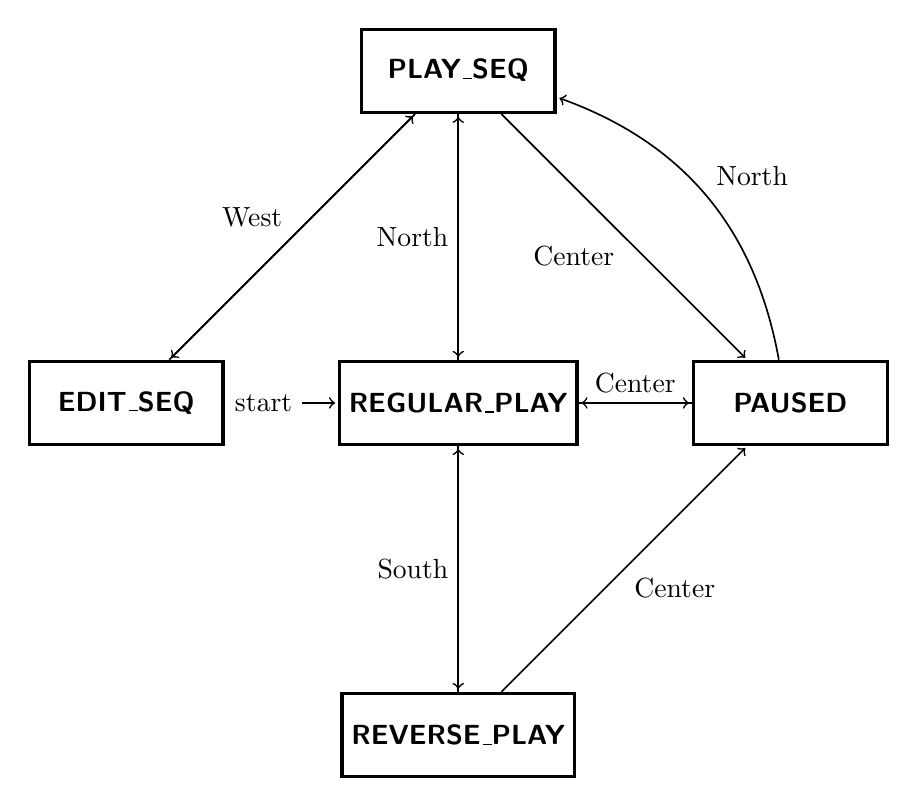
\begin{tikzpicture}[shorten >=1pt, node distance=10cm,on grid, auto, semithick]
	\tikzstyle{state} = [draw, very thick, fill=white, rectangle, minimum height=3em, minimum width=7em, node distance=12em, font={\sffamily\bfseries}]
	\tikzstyle{stateEdgePortion} = [black,thick];
	\tikzstyle{stateEdge} = [stateEdgePortion,->];
	\tikzstyle{edgeLabel} = [pos=0.5, text centered, font={\sffamily\small}];
	
	\node[state,initial](rp) {REGULAR\_PLAY};
	\node[state](revp) [below =of rp]{REVERSE\_PLAY};
	\node[state](p) [right=of rp]{PAUSED};
	\node[state](playseq) [above=of rp]{PLAY\_SEQ};
	\node[state](editseq) [left=of rp]{EDIT\_SEQ};
	
	\path[->]
	(playseq) edge node [swap] {Center} (p)
		edge node [swap] {West} (editseq)
		edge node {} (rp)
	(editseq) edge node {} (playseq)
	(rp) edge node {Center} (p)
		edge [swap] node {South} (revp)
		edge node {North} (playseq)
	(p) edge node {} (rp)
		edge [bend right, swap] node {North} (playseq)
	(revp) edge [swap] node {Center} (p)
		edge [swap] node {} (rp);
	\end{tikzpicture}
\end{center}

We have added two new states \verb|PLAY_SEQ| and \verb|EDIT_SEQ|. You should wire up the west compass LED to \verb|current_state == EDIT_SEQ| and the north compass LED to \verb|current_state == PLAY_SEQ|. You should implement the skeleton of this state machine before proceeding with the complete explanation.\\

Our goal is to create an 8-tap music sequencer that we can use along with our regular music streamer. Our music sequencer will have a place (RAM) where it stores the \verb|tone_switch_period|s of 8 notes. When we are in the \verb|PLAY_SEQ| state, the music streamer will play the 8 notes, one after the other, in a continuous loop. Each note will play for a set amount of time as determined by the \textbf{sequencer tempo}. While in the \verb|PLAY_SEQ| state we can change the sequencer tempo using the rotary encoder (\textbf{the sequencer tempo is different from the ROM tempo you modified earlier})

We can edit these 8 notes on the fly by moving into the \verb|EDIT_SEQ| state. In this state, the LEDs will show which of the 8 notes we are currently editing. By spinning the rotary encoder, we can select a new pitch for this note. By clicking in the rotary encoder, we can save the selected pitch in the RAM location for this note. We can use the east and west buttons to edit a different note.\\

You will find some skeleton code in \verb|lab4/src/music_streamer.v| to help you implement the sequencer. This is a complicated circuit, so you should add features slowly and modify the \verb|tone_generator_testbench| to test out your sequencer. Here is a list of requirements for your sequencer:

\begin{enumerate}
	\item You should have two tempo controls. 
	
	\begin{enumerate}
		\item The \textbf{ROM tempo} affects the duration of each note in the ROM and can be modified in either the \verb|REGULAR_PLAY| or \verb|REVERSE_PLAY| states by the rotary encoder.
		\item The \textbf{sequencer/RAM tempo} affect the duration of each note in the sequencer RAM and can be modified only in the \verb|PLAY_SEQ| state by the rotary encoder.
	\end{enumerate}
	
	\item The GPIO leds should be used for the following functions in different states.
	
	\begin{enumerate}
		\item In the \verb|REGULAR_PLAY|, \verb|PAUSED|, and \verb|REVERSE_PLAY| states, the 8 GPIO LEDs should display the top 8 bits of the ROM address.
		\item In the \verb|PLAY_SEQ| state, the 8 GPIO LEDs should display the note being played. For example, if note 5 is currently being played, LED 5 should be on and the rest off.
		\item In the \verb|EDIT_SEQ| state, the 8 GPIO LEDs should display the note being edited. For example, if we are editing note 6, LED 6 should be on and the rest off.
	\end{enumerate}
	
	\item In the \verb|EDIT_SEQ| state, the piezo speaker should play the current pitch of the note. Spinning the rotary encoder should increase and decrease the pitch by some amount per click that you determine. Pressing the rotary encoder button should save the current pitch of the note into the sequencer's RAM.
	
	\item In the \verb|EDIT_SEQ| state, pressing the east or west buttons should change the note being edited. As you change notes, the piezo speaker should play the pitch of the new note being edited.
	
	\item You can use the same \verb|clock_counter| for all parts of this state machine including the sequencer and the regular music streamer.
	
	\item You can use the same \verb|sequencer_address| for the two sequencer states.
	
	\item You can choose what the reset values for the sequencer RAM entries are. A sensible default is provided in the skeleton code.
\end{enumerate}

Please ask the TA if you have any questions about specifications for the sequencer or FSM in general.

\section{Conclusion + Checkoff}
You are done with lab 4! Please write down any and all feedback and criticism of this lab and share it with the TA. This is a brand new lab and we welcome everyone's input so that it can be improved.\\

\subsection{Checkoff Tasks}

\begin{enumerate}
	\item Show the TA your working design with the FSM. Be able to transition states by clicking on the north and center buttons and show that your \verb|music_streamer| matches the spec.
	
	\item Show the tempo control working by spinning the rotary encoder to speed up and slow down the music.
	
	\item Demonstrate that hitting the \verb|CPU_RESET| button resets the ROM address back to 0 and puts the FSM into the \verb|REGULAR_PLAY| state.
	
	\item Demonstrate that you can transition into the \verb|SEQUENCER| state and that you can edit your tones and play them back. 
	
	\item Show the TA your Verilog RTL for all the components you designed for this lab (synchronizer, debouncer, rotary decoder, FSM) and briefly explain the design of each of them.
\end{enumerate}

\end{document}